
\section{\textcolor{black}{UQ framework and components}}
%------------------------------------------------
\begin{frame}
\frametitle{Experiments, Models, Simulations, and UQ}
\begin{figure}
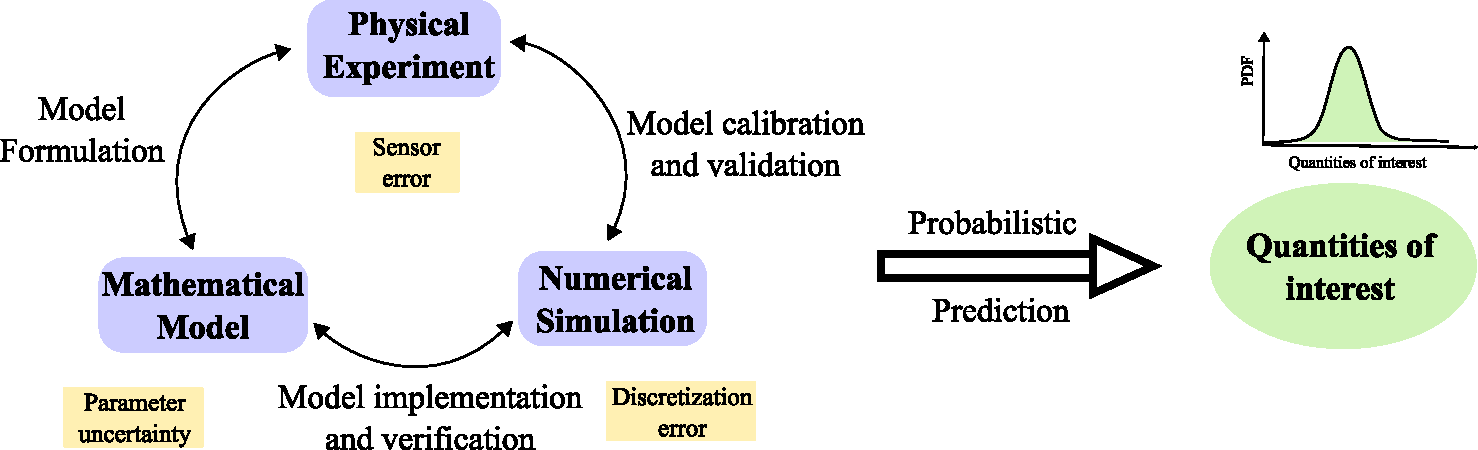
\includegraphics[scale=0.6]{figures/figure-UQ_physics_Model_Simulation.pdf}
\end{figure}
\end{frame}

%------------------------------------------------
\begin{frame}
\textbf{\frametitle{UQ problems and components}
\only<1>{
\begin{figure}
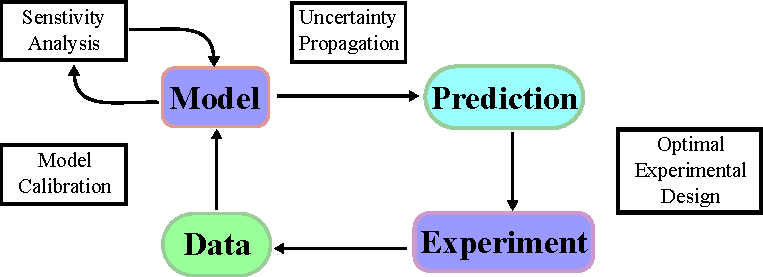
\includegraphics[scale=0.9]{figures/figure-UQ_components.pdf}
\end{figure}}
}
\only<2>{
\begin{block}{Two UQ types of problems:}
  \begin{figure}
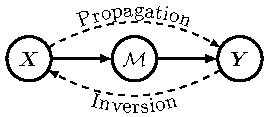
\includegraphics[width=6.5cm]{figures/figure_UQ_propagation_inversion.pdf}
\end{figure}  
\end{block}
\begin{block}{Four components:}
\begin{enumerate}
    \item Uncertainty propagation
    \item Model calibration
    \item Sensitivity analysis
    \item Optimal experimental design
\end{enumerate}  
\end{block}

}

\end{frame}

%------------------------------------------------
\begin{frame}
\framesubtitle{} % Optional subtitle
\begin{definition}
  A computational model should contain:
    \begin{itemize}
        \item a \alert{mathematical description} of the physics 
        \item may be seen as a \alert{black box} to compute the QoI
    \end{itemize}
\end{definition}
\only<1>{
        \begin{figure}            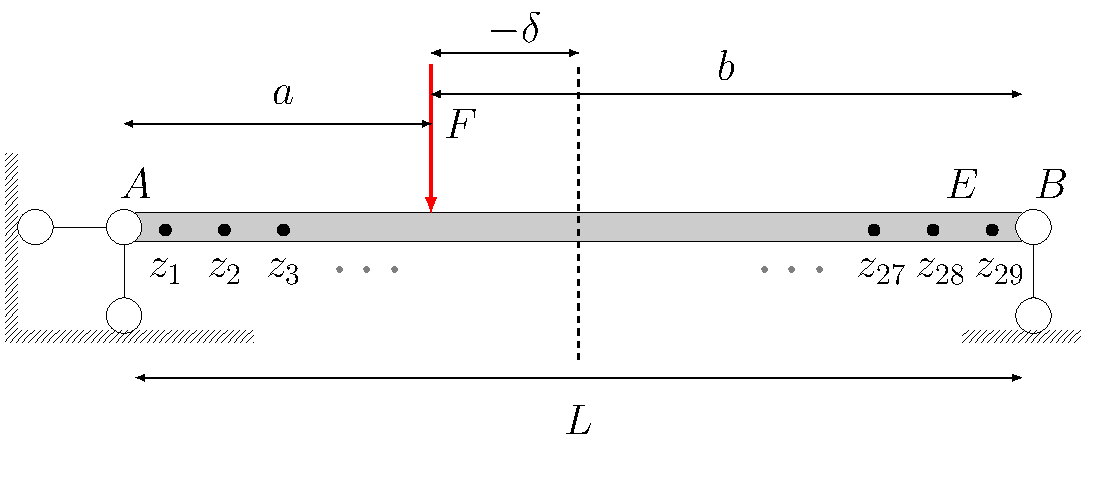
\includegraphics[scale=0.4]{figures/figure-beam.pdf}
        \end{figure}          
        \begin{equation}
                    y = \left\{\begin{matrix}
        \frac{F b  x  [(L^2 - b^2) - x^2]}{6LEI}  \ x \le a
         \\
         \frac{F b  [\frac{L}{b} (x - a)^3 + (L^2 - b^2)]}{6LEI} \ x> a
        \end{matrix}\right.
        \end{equation}
        }
        
\only<2>{
\begin{figure}
    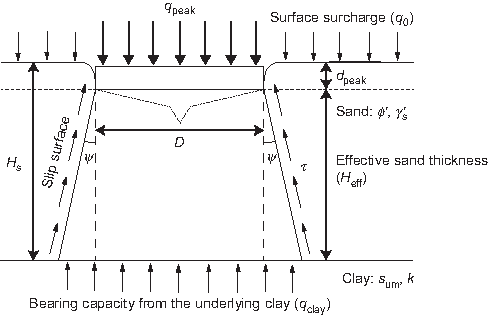
\includegraphics[scale=0.8]{figures/figure-qpeak.pdf}\footfullcite{li2018}
\end{figure}
}

\only<3>{
\bigskip
Numerical methods:
\begin{itemize}
    \item Finite element method
    \item Finite difference method
    \item $\cdots$
\end{itemize}
}
\end{frame}

%------------------------------------------------------------------------------------------------------------------------




%-----------------------------------------------------------------------------------------------------------------------
\begin{frame}
 \frametitle{UQ components one-Uncertainty propagation}
 \only<1>{
 \begin{figure}
    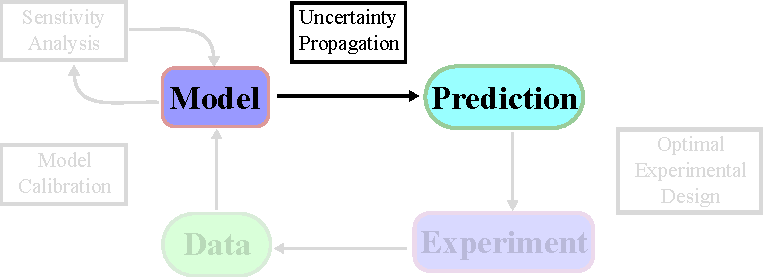
\includegraphics[scale=0.9]{figures/figure-UQcomponetone-propagation.pdf}
\end{figure}
\begin{itemize}
    \item \alert{Uncertainty propagation} feeds quantified input uncertainties through our model to produce probabilistic predictions of a QoI
\end{itemize}
 }

 \only<2>{
 \begin{figure}
    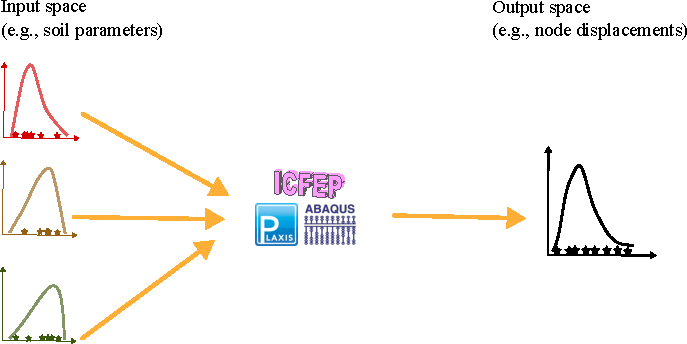
\includegraphics[scale=0.9]{figures/figure-UQ_propagation_MC.pdf}
\end{figure}
\begin{itemize}
\setlength\itemsep{0.5cm}
\item \alert{Output statistics}, i.e., mean, standard deviation. etc.
\begin{equation*}
    \mu_{\boldsymbol{Y}} = \mathbb{E}_{\boldsymbol{X}}
[\mathcal{M}(\boldsymbol{X}) ]; \ 
\sigma^2_{\boldsymbol{Y}} = \mathbb{E}_{\boldsymbol{X}}
[(\mathcal{M}(\boldsymbol{X}) - \mu_{\boldsymbol{Y}})^2]
\end{equation*}
\item \alert{Distribution} of the QoI
\item \alert{Probability} of exceeding an admissible threshold $y_{adm}$ following $P_{f} = \mathbb{P}(\boldsymbol{Y} \ge y_{adm})$
\end{itemize}
 }



 \end{frame}

 %---------------------------------------------------------------------------------------------------
\begin{frame}
 \frametitle{UQ components two-Model calibration}
 \only<1>{
 \begin{figure}
    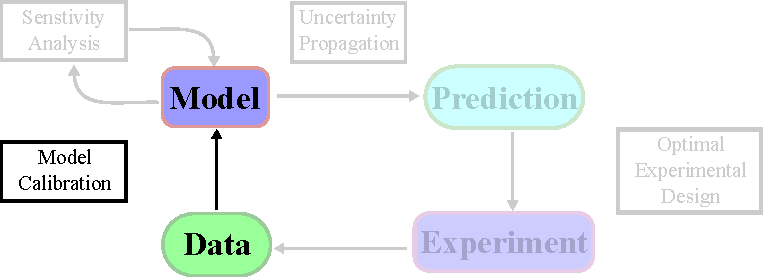
\includegraphics[scale=0.9]{figures/figure-UQcomponetwo-calibration.pdf}
\begin{itemize}
    \item \alert{Model calibration} explicitly quantifies model input uncertainties using experimental data (improve/update initial assumptions)
\end{itemize}
\end{figure}
 }

 \only<2>{
 \framesubtitle{Choice for UQ inversion}
\begin{columns}
    \column{0.5\textwidth}
        Choice for the UQ method is totally based on the {\textcolor{red}{\textbf{quantity}}} of accessible data:
        \begin{itemize}
            \item  {\textcolor{red}{\textbf{Lack}}} or {\textcolor{red}{\textbf{no}}} data available, model can be solely based on expert judgement
            \item {\textcolor{red}{\textbf{Substantial}}} volume data available, model can fully use statistical inference (e.g., the methods of moments)
            \item {\textcolor{red}{\textbf{Combination}}} of two above: Bayesian methods
            \begin{equation*}           \pi(\boldsymbol{x}|\mathcal{Y}) = \frac{{\mathcal{L}(\boldsymbol{x}|\mathcal{Y}) \cdot \pi(\boldsymbol{x})}}{{\pi(\mathcal{Y})}} 
            \end{equation*}
        \end{itemize}
    
    \column{0.5\textwidth}
        \begin{figure}[!ht]      
        %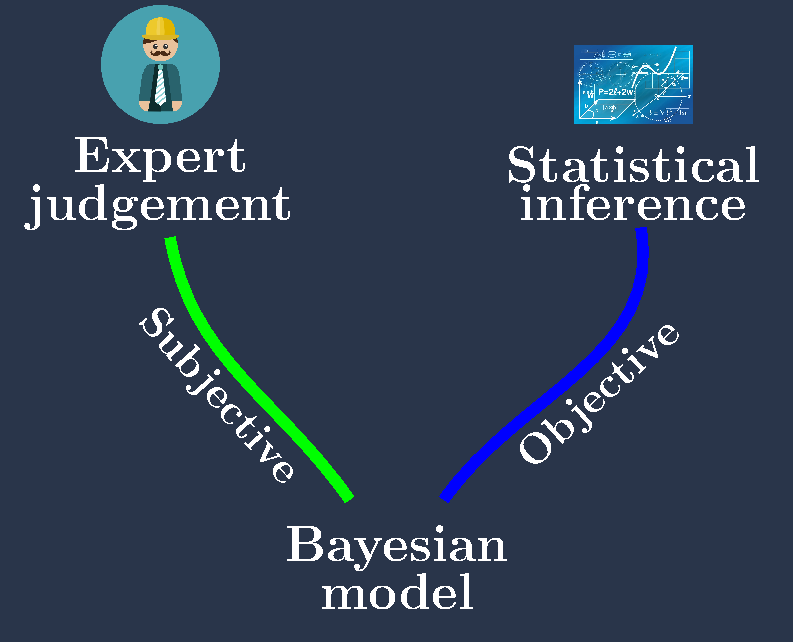
\includegraphics[scale=0.6]{figures/figure_objvssub.pdf}
        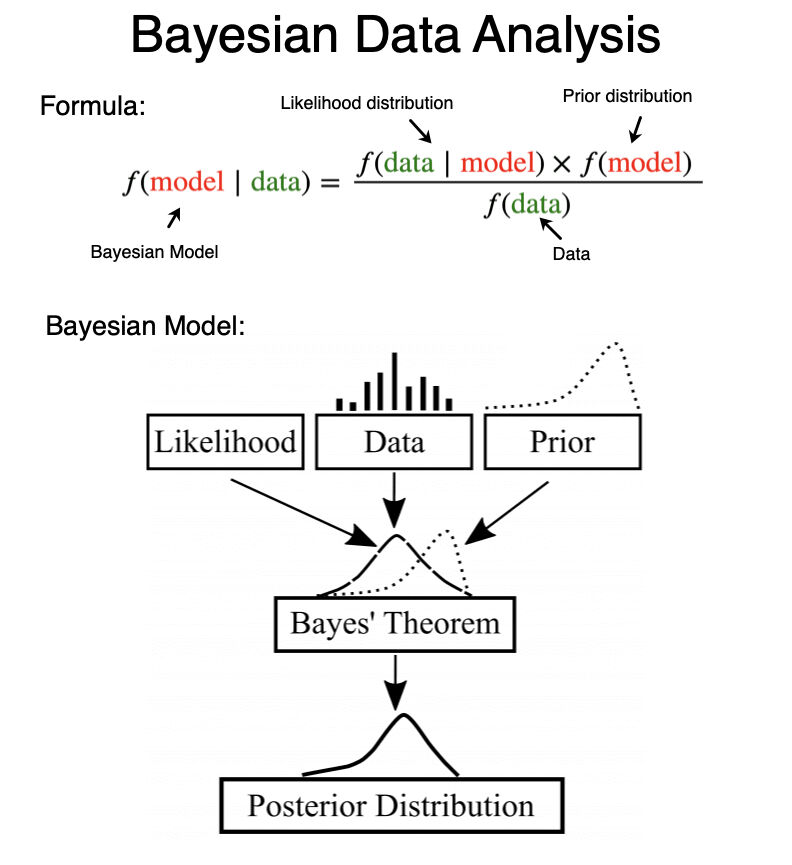
\includegraphics[scale=0.22]{figures/figure_Bayesflow.jpg}
        \end{figure}
\end{columns}
 }


\only<3>{
\begin{block}{Bayesian methods}
    Expert guess + Limited data $\rightarrow$ Distribution
\end{block}
\begin{columns}
    \column{0.5\textwidth}
    Prior:
    \begin{figure}[!ht]       
    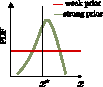
\includegraphics[scale=2]{figures/figure-weakandstrongprior.pdf}
    \end{figure}
    
    \column{0.5\textwidth}
    Likelihood:
    \begin{figure}[!ht]       
    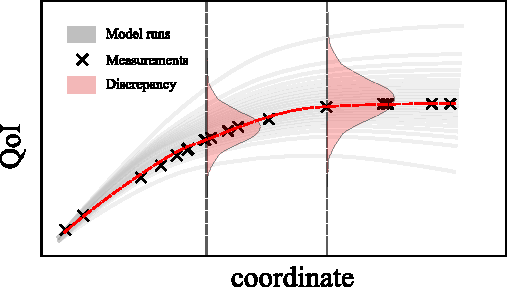
\includegraphics[scale=0.6]{figures/figure-likelihood.pdf}
    \end{figure} 
\end{columns}
\begin{alertblock}{Notable caveats:}
\begin{itemize}
    \item Prior-Requires specific expertise
    \item Likelihood-Computationally expensive 
\end{itemize}  
\end{alertblock}
}



 \end{frame}
 %======================================================================================================

 %---------------------------------------------------------------------------------------------------
\begin{frame}
 \frametitle{UQ components three-Sensitivity analysis}

 \only<1>{
 \begin{figure}
    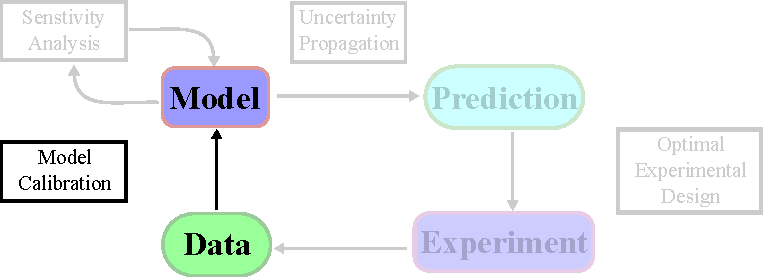
\includegraphics[scale=0.9]{figures/figure-UQcomponetwo-calibration.pdf}
\begin{itemize}
    \item \alert{Sensitivity analysis} identifies the most influential parameters
\end{itemize}
\end{figure}
 }
 
 \only<2>{
 \begin{quote}
   \Large Sensitivity analysis-Determine what are the input parameters whose uncertainty explains the variability of the QoI   
 \end{quote}{}


\begin{columns}
    \column{0.6\textwidth}
    \begin{itemize}
        \item detect input parameters whose uncertainty has \alert{no impact} on the output variability
        \item detect input parameters which allow one to best \alert{decrease the output variability} when set to a deterministic value
        \item detect \alert{interactions} between paramters
    \end{itemize}
    \column{0.4\textwidth}
\begin{figure}          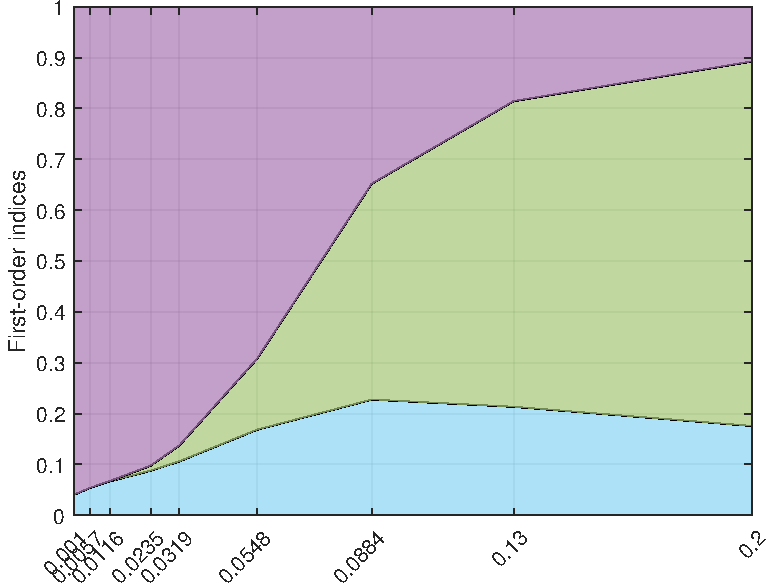
\includegraphics[scale=0.45]{figures/figure-Sobol.pdf}
\end{figure} 
\end{columns}
 }

\only<3>{
\begin{block}{Total variance:}
\begin{equation*}
D\equiv \text{Var}[\mathcal{M}(\boldsymbol{X}) ]
= \text{Var}[\sum_{u \subset \{1,\cdots,M\}} \mathcal{M}_{u}(\boldsymbol{X}_{u}) ]
= \sum_{u \subset \{1,\cdots,M\}} \text{Var}[\mathcal{M}_{u}(\boldsymbol{X}_{u}) ] 
\end{equation*}    
\end{block}

\begin{itemize}
    \item Sobol's indice:
    \begin{equation*}
S_u   \overset{\mathrm{def}}{=} \frac{\text{Var}[\mathcal{M}_{u}(\boldsymbol{X}_{u}) ] }{D} 
    \end{equation*}

    \item First-order Sobol's indice:
     \begin{equation*}
S_i = \frac{D_i}{D} = \frac{\text{Var}[\mathcal{M}_{i}(\boldsymbol{X}_{i}) ] }{D}
    \end{equation*}
    Quantify the effect of each input parameter \alert{separately}

    \item Total Sobol's indice:
    \begin{equation*}
S_{i}^{T} \overset{\mathrm{def}}{=}  
\sum_{u \supset i} S_u
    \end{equation*}
    Quantify the \alert{total effect} of $x_{i}$, including \alert{interactions} with other variables
\end{itemize}
}

 \end{frame}
 %--------------------------------------------------------------------------------------------------
\begin{frame}
 \frametitle{UQ components three-Optimum Experimental design}
 \only<1>{
 \begin{figure} 
 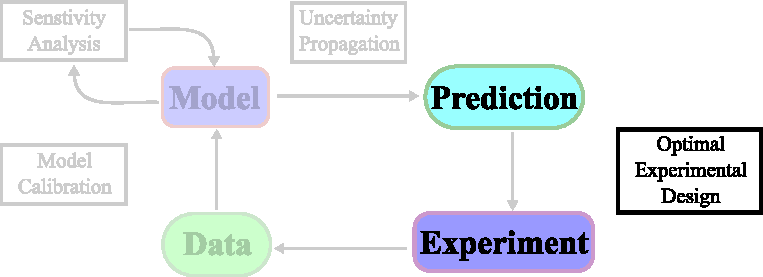
\includegraphics[scale=0.9]{figures/figure-UQcomponent_ActiveLearning.pdf}
\end{figure} 
 }

 \only<2>{

  \begin{figure} 
 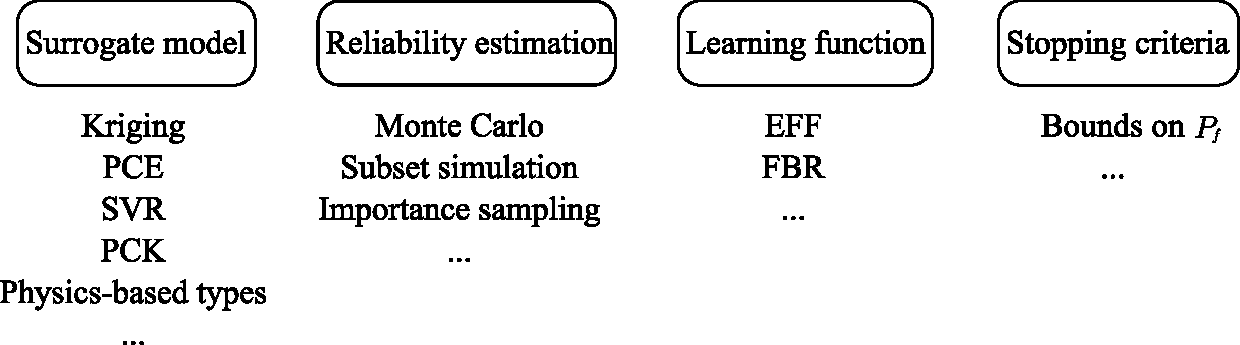
\includegraphics[scale=0.6]{figures/figure-activeLearning_idea.pdf}
\end{figure}
\begin{columns}
    \column{0.5\textwidth}
      \begin{figure} 
 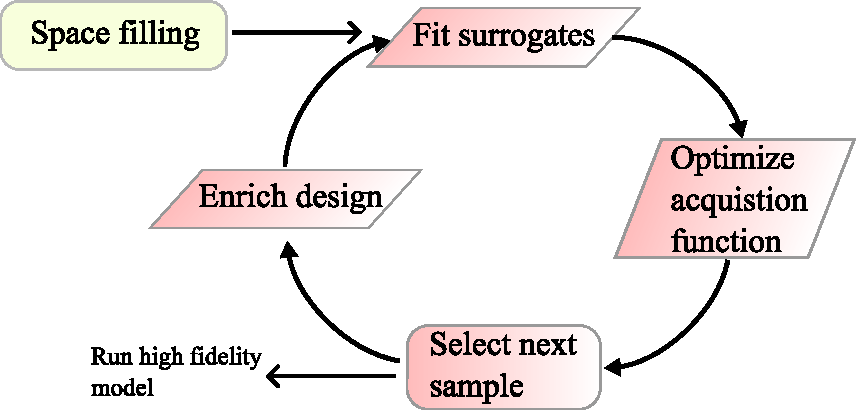
\includegraphics[scale=0.4]{figures/figure-activeLearning_chart.pdf}
\end{figure}
    \column{0.5\textwidth}
    \begin{block}{}
    \begin{itemize}
        \item Not each run is equally important
        \item Save time
    \end{itemize}       
    \end{block}
 
\end{columns}
 }
 \end{frame}
 %--------------------------------------------------------------------------------------------------


 
\begin{frame}
\frametitle{Uncertainty quantification for engineering problems}
Research topics
\begin{itemize}
    \item \textcolor{red}{Uncertainty modelling for engineering systems}
    \item \textcolor{red}{Bayesian model calibration}
    \item Structural reliability analysis
    \item Surrogate models (low dimensions/high dimensions)
    \item Stochastic inverse problem
    \item Global sensitivity analysis
    \item Reliability-based design optimization
    \item ...
\end{itemize}

\end{frame}




